\subsubsection{25.01.16}
Today we discussed improvements that we need make in our robot
Problems and solutions for each module:
	\begin{enumerate}
		\item Wheel base:
		\begin{table}[H]
			\vspace{-2mm}
			\begin{center}
				\begin{tabular}{|p{0.15\linewidth}|p{0.4\linewidth}|p{0.55\linewidth}}
					\hline
					Problem & Solution\\
					\hline
					Cudes gets under the wheels & To make protection for wheels \\
					\hline
					Small wheels dents when robot try ride trough the churro & To fill tires with something rigidly\\
					\hline
					The beam on which fixed axles of wheels hook churro & To cut it
				\end{tabular}
			\end{center}
		\end{table}
		\item Lift and bucket:
		\begin{table}[H]
			\vspace{-2mm}
			\begin{center}
				\begin{tabular}{|p{0.15\linewidth}|p{0.4\linewidth}|p{0.55\linewidth}}
					\hline
					Problem & Solution\\
					\hline
					MIL isn't finished  & Finish it when we'll get necessary elements\\	
					\hline
				\end{tabular}
			\end{center}
		\end{table}
		\item Gripper for debris - no problems.
		\item Mechanism for scoring climbers - no problems.
		\item Programme of autonomous period - no problems.
		
		\item In addition we need mount NXT lower because mechanism for scoring climbers hook it. 
		
		\item Also we need to remake electricity for new Android platform when we'll get Android devices, Core power module and controllers.
	\end{enumerate}
\begin{itemize}
	\item Wheels were filled with cardboard.
	
	\item The beam that hook churro was cut.
	
	\item After this improvements robot was able to ride through first churro by two wheel pairs. But the front wheel pair can't do it. We thought that if we'll install caterpillar on front wheels or small rollers that will rise them robot will be able climb to middle zone. But it was decided test it after completing all rest tasks.
	\subsubsection{26.01.16}	
		\item Today we got necessary elements for mounting bucket and turning mechanism for it. It was found that during elaborating of lift it was made a mistake in estimating of beam's length (necessary length is smaller on 0.5cm). So we need to rise the lift. But in this case we need change transmission (install smaller gears) because else height of robot will be more than 45.72cm.
		\begin{figure}[H]
			\begin{minipage}[h]{1\linewidth}
				\center{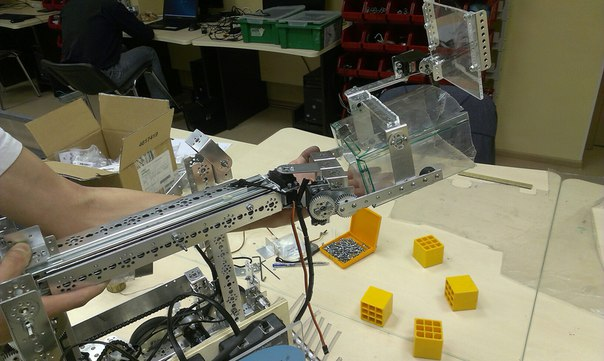
\includegraphics[scale=0.5]{days_L/Meetings/images/17}}
				\caption{Mount of bucket}
			\end{minipage}
		\end{figure}
		
		\item It was installed the protection for wheels.
		
		\item NXT was fixed lower.
	\subsubsection{27.01.16}
		\item It was decided make transmission 8:1 (three-stage transmission each stage - 2:1). It allowed us to mount rotation axis of moving beam of lift higher. 
		\begin{figure}[H]
			\begin{minipage}[h]{1\linewidth}
				\center{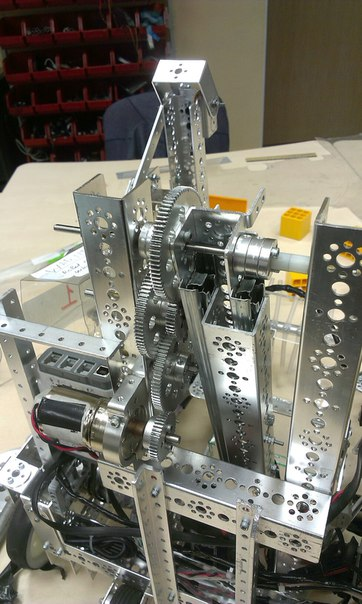
\includegraphics[scale=0.5]{days_L/Meetings/images/16}}
				\caption{New transmission}
			\end{minipage}
		\end{figure}
	\subsubsection{28.01.16}
		\item Servos were connected to controllers.
	\subsubsection{30.01.16}
		\item Today we got servo for MEL. MEL was assembled but during test it was found that servo is not able to extract lift. We need install second servo or invent other solution.		
		\item Also it was found that motor that turn lift can't do it when it extracted. Maybe that's because of the failure of the motor.
	\subsubsection{01.02.16}		
		\item It was installed Andy Mark motor for turning lift. It can move it even if lift extracted.
		\item It was invented MEL with blocks.
		\item Reel for MEL and servo that rotate it were installed. The rope wasn't installed because we hadn't it today.
	\subsubsection{03.02.16}
		\item They were fixed blocks and rope for MEL. MEL was tested. Result is positive: servo is able to extract lift in 2 seconds.
	\subsubsection{04.02.16}
		\item They were hold wires for servos.		
\end{itemize}		
\fillpage